\chapter{Proteus is Turing Complete}\label{chapter:ProteusTC}

This section will describe how we will construct the proof showing that Proteus is TC.

\section{Useful information to be used in the proof}

First, I will discuss features about Proteus programs on a theoretical level.
Then, I will discuss features about the Proteus language that allow for the creation of a TM.
This is the background information that will guide the construction of the proof outline and ultimately the proof itself.

\subsection{Undecidable input}\label{subsec:UndecidableInput}

Because Proteus is a higher-level programming language, we can leverage the usage of Rice's Theorem, Theorem \ref{thm:RiceThm}.
Thus, given any input it is impossible to determine an answer to the Halting Problem.
Furthermore, one cannot determine if there is an actor that will be told to switch to a particular state.
With this knowledge, it is understood that any given Proteus program is undecidable.
Thus, I will look at how to create a TM in Proteus.

\subsection{Requirements of a TM}\label{subsec:ReqsofTM}

In this section, I will point out critical pieces of Proteus that prove useful to create a TM.
We can see that the core features to create a TM, seen previously in sections \ref{subsec:TMLogicalDesign} and \ref{subsubsec:ProgCalc}, include:
\begin{enumerate}
    \item Arithmetic and Logical Processing
    \item Memory storage and manipulation
    \item Conditional Logic
    \item Looping Logic
    \item Input/Output
\end{enumerate}

Recall the proteus grammar seen in section \ref{subsec:ProteusGrammar}.
I will now describe from the Proteus grammar how to construct/use Proteus creating each part of the TM.

\subsubsection{Arithmetic and Logical Processing}\label{subsubsec:ArithLogProc}

The grammar provides the following definitions for arithmetic and logical processing:
\begin{itemize}
    \item BinOp
    \item Type
    \item ConstExpr
\end{itemize}

'BinOp' handles all binary operations for both arithmetic and logical calculation.
Some features include addition, subtraction, multiplication, division, modular arithmetic, equivalence relations, and, and or.
Looking at brainfuck in section \ref{subsubsec:EsotericPL}, one can notice that the only necessary mathematical operations are addition and subtraction.
Furthermore, the only logical processing is seen in the looping mechanism.
If the value at the pointer is 0 and the input token is a '[', then the loop is skipped.
This means that there is an equality check which returns a boolean result.

Looking deeper at the types of Proteus, type consists of all the possible types that are built into the language:
\begin{itemize}
    \item int
    \item string
    \item boolean
    \item actorname
    \item statename
    \item eventname
\end{itemize}

Despite allowing for division, the set of integers is closed under truncation, which is how Proteus handles cases where normally it wouldn't be.
eg. 5 / 2 = 2.5, but under truncation 5 / 2 = 2.
These truncation rules are similar to those seen in other languages such as Java and C \cite{TruncJava,TruncC}.

'ConstExpr' describes the 3 simple data types: Int, String, and Boolean.
These 3 types are capable of mimicking the behavior of brainfuck as well.

\subsubsection{Memory Storage and Manipulation}\label{subsubsec:MemStoManip}

The grammar provides the following definitions for memory storage and manipulation:
\begin{itemize}
    \item DefHSM
    \item DefState
    \item DefGlobalConst
    \item DecStmt
    \item AssignStmt
    \item SendStmt
\end{itemize}

'HSM' are Hierarchical State Machines which are actors in the language.
These state machines utilize states to determine logical processing.
These logical processes may utilize local or global variables that are stored, via the 'DecStmt' and 'DefGlobalConst' definitions respectively.

To modify data, the 'AssignStmt' was defined which allows for modifying the value of a given variable.
State Machines can modify state via the 'SendStmt' command.
Utilizing 'SendStmt', state machines can modify the state of themselves and other state machines as well.

\subsubsection{Conditional Logic}\label{subsubsec:CondLog}

The grammar provides the following definitions for conditional logic:
\begin{itemize}
    \item GoStmt
    \item JustGoStmt
    \item GoIfStmt
    \item ElseGoStmt
    \item IfStmt
\end{itemize}

Conditional Logic or Branching is necessary for a TM to compute any calculable function (see: Theorem \ref{thm:CTT}).
'GoStmt' is considered either a 'JustGoStmt' or a 'GoIfStmt', which are used to switch between states of a given HSM.
Similarly, the 'ElseGoStmt' switches to a particular state of a given HSM if the condition from the 'GoIfStmt' fails.

The 'IfStmt' is utilized for conditional logic within the processing of the state machines, and is akin to the standard if statements in other programming languages.
It is defined recursively to allow for nested "If ... else if.... else ..." statements.
These definitions allow for conditional statements to occur for a given HSM and within the code itself.

\subsubsection{Looping Logic}\label{subsubsec:LoopLog}

The only looping logic that can be seen in the garmmar that is built in, is the:
\begin{itemize}
    \item WhileStmt
\end{itemize}

This is the only necessary form of looping, as it can be broken by conditional statements and is capable of performing like other loops such as the do-while, for, and so forth.
This allows for more complex logical processing, such as recursion, which is a necessary requirement for TMs to perform any calculation.
A simplistic example of a problem that requires recursion would be the Ackermann Function.
See the definition of the Ackermann function here:
\[
\begin{aligned}
    A(0, n) &= n + 1\\
    A(m + 1, 0) &= A(m,1)\\
    A(m + 1, n + 1) &= A(m,\hspace{0.1cm} A(m + 1,n))
\end{aligned}
\]

Although being able to compute the Ackermann function requires recursion, it doesn't conclude that any system that can compute it is TC.
It was created to show that not all total computable functions are primitively recursive \cite{AckermannPR}.
The Ackermann function exists to show that not all functions can be represented with for loops, which is what primitive recursive functions are \cite{RecursiveFuncs}.
Nonetheless, all computable functions (regardless of their expression) are capable of being calculated by a TM, as stated by the Church-Turing Thesis (Theorem \ref{thm:CTT}).

\subsubsection{Input/Output}\label{subsubsec:IO}

Looking at the grammar definitions for:
\begin{itemize}
    \item Stmt
    \item PrintlnStmt
    \item PrintStmt
    \item SendStmt
\end{itemize}

From 'Stmt' I would like to highlight the 'SendStmt' command.
'SendStmt' is utilized to send events to a particular State Machine (i.e. an output).
By default, all actors are able to receive events.
'PrintlnStmt' and 'PrintStmt' are the standard print and println commands that are well known from other languages which serve as output to the console.
Although there is no explicit way to allow for input from the systems grammar dynamically, this is unnecessary as it can be preconfigured before runtime.
Thus, there exists a way to send inputs before the program is run via static input of values.

\section{Proteus Turing Machine Description}\label{sec:ProteusTMDescr}

By showing that any input to Proteus programs are undecidable and it is possible to create a TM in Proteus, Proteus can be shown to be TC.
This proof leverages the usage of both the Church-Turing Thesis, Theorem \ref{thm:CTT}, and Rice's Theorem, Theorem \ref{thm:RiceThm}.

I will explicitly create a TM using the built-in features seen previously in section \ref{subsec:ReqsofTM}.
After showing how to create a TM within Proteus, I will use Proteus to implement Conway's Game of Life and Rule 110 .
This is to demonstrate that the system is TC.
Recall demonstrating an implementation of CGoL or Rule110 indicates the system is TC from sections \ref{subsubsec:CGoL} and \ref{subsubsec:Rule110}.

\begin{enumerate}
    \item Define the set of internal states
    \item Define the initial state
    \item Define the final state
    \item Define the input alphabet
    \item Define the tape alphabet
    \item Define the state transitions
    \item Define the blank symbol
\end{enumerate}

I will now describe how to create a TM within Proteus from a higher abstraction layer with section \ref{sec:DefnTMProteus} going into the formal definition.
The tape is a series of state machines, HSMs, that will be ordered as $c_{0}, c_{1}, \dots , c_{\text{n}}$ arbitrarily with $c_{\text{n}}$ being the last non-empty cell.
This order will be consistent and not allow state machines to swap places with each other in the sequence.
There will be an additional state machine which functions as the read/write head.
The read/write head will be the one describing what the state of the TM and overall program is.
It contains a queue of events to be broadcast, with each entry in the queue containing a single event and target state machine.
Whenever a non-empty cell is encountered by the read/write head, it will broadcast what the current state is.
Figure \ref{fig:ProteusTMDesign} shows the design of the TM in a simplified manner.

\begin{figure}[h!]
    \centering
    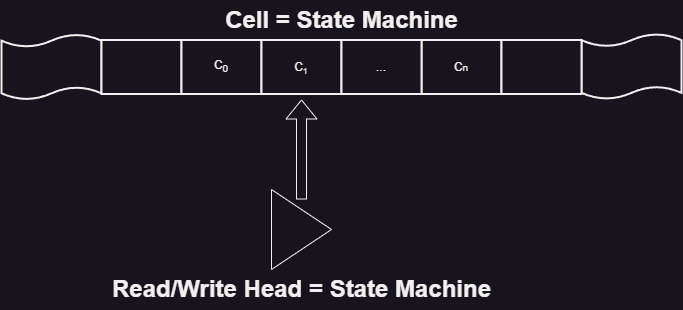
\includegraphics[width=16cm]{images/ProteusTMDesign.png}
       \caption{Design of TM in Proteus}
           \label{fig:ProteusTMDesign}
\end{figure}

When the Proteus program is run, the read/write head will enter the 'ProgramOn' State.
If the tape is empty, as in there are no state machines that are created by the programmer, then the read/write head enters the 'ProgramOff' state and halts.
If instead the cell is non-empty, then the read/write head enters the 'Read' state which begins the process of reading information from the tape.
If a write is to be issued, then the read/write head enter the 'Write' state and writes the new data in the current cell.
After the write, the read/write enters the 'Read' state once again.

The logic for movement to an adjacent cell is mirrored on the left and right sides.
I will describe the movement to the left-adjacent cell.
From the current cell, the read/write head enters the 'BoundLeft' state and determines whether it encounters another symbol or the blank.
If there is a symbol, then it still lies within the non-empty tape information and returns to the 'Read' state.
If instead there is a blank, this means that there is no state machine defined, and has extended past the bounds of the tape with given information.
The read/write head moves one cell to the right, then returns to the 'Read' state to continue processing.
Because Proteus does not allow for dynamic state machine creation, the read/write head leaves the blank unmodified along the tape.

To exit the program and enter the halting state, all state machines within the tape must enter the 'Off' state, indicated by the 'O' within Figure \ref{fig:ProteusStateTM}.
The read/write head enters the 'FindStart' state from the 'Read' state to prepare for halting.
In the 'FindStart' state, the read/write head will move to the left, one cell at a time.
When it encounters a blank cell, it moves the read/write head to the adjacent right cell and enters the 'Check' state.
In the check state, the read/write head moves one cell at a time to the right and checks if they are in the 'Off' state.
Upon encountering a cell that is not in the 'Off' state the read/write head enters the 'Read' state for further processing.
If every cell is in the 'Off' state, then the read/write head will encounter a blank on the next cell after $c_{\text{n}}$.
In this case, all state machines are in the 'Off' state and the read/write head enters the 'ProgramOff' state to halt.

Because the read/write head is itself a state machine, it contains an event queue for events to be broadcasted.
Each event is associated to a single state machine.
In order to find the proper state machine to send the event to, the read/write head must search for it within the bounds of the non-empty tape.
This searching cannot utilize 'FindStart', because if all state machines are off and there are some nonzero number of events still in the queue, then the machine will still have events to process, but end up in the 'ProgramOff' state.
As such, it must search for them and find them using an unoptimized algorithm such as brute forcing all possible movements across the non-empty tape.
Note that I will explicitly describe what values $x, y, \text{O}$ must be in the following section \ref{sec:DefnTMProteus}.

\begin{figure}[h!]
    \centering
    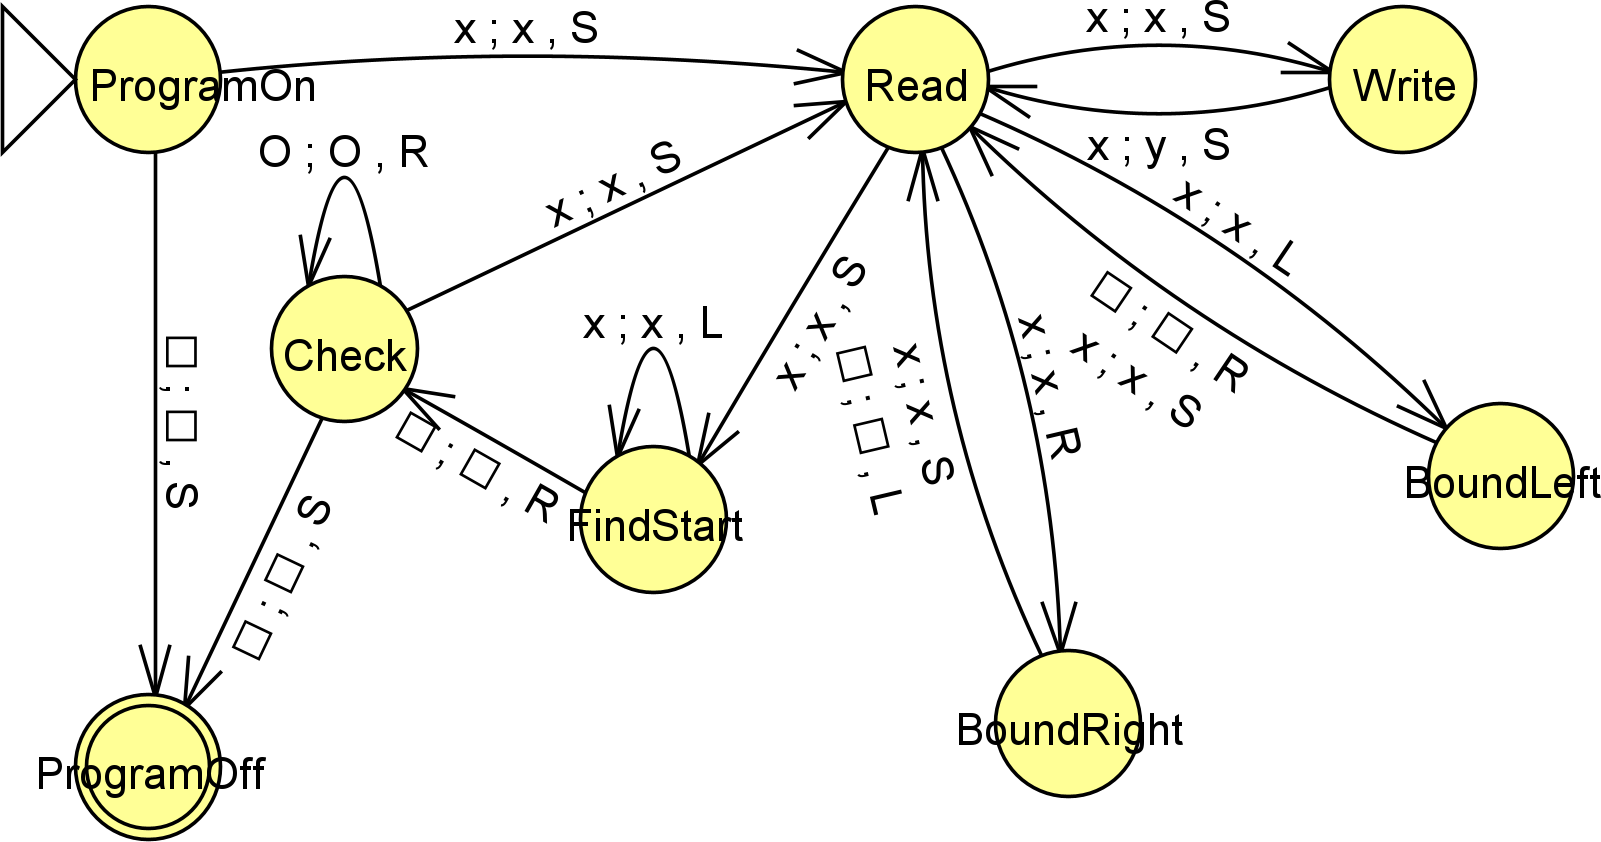
\includegraphics[width=16cm]{images/ProteusTM.png}
       \caption{TM State Diagram in Proteus}
           \label{fig:ProteusStateTM}
\end{figure}

\section{Definition of a Turing Machine in Proteus}\label{sec:DefnTMProteus}

The list of internal states describes the states that the read/write head has.
The list of states is seen in Figure \ref{fig:ProteusStateTM} and will be described formally below.
\[
Q = \{\text{'ProgramOn'}, \text{'ProgramOff'}, \text{'Read'}, \text{'Write'}, \text{'BoundLeft'}, \text{'BoundRight'}, \text{'FindStart'}, \text{'Check'}\}
\]

The initial state of the program is 'ProgramOn', thus \[q_{0} = \text{'ProgramOn'}.\]

There is only a single halting state, 'ProgramOff'.
Therefore, the set of Final states is written, \[F = \{\text{'ProgramOff'}\}.\]

The input alphabet consists of the symbols that appear as already existing on the tape.
Recall that each cell is a state machine in Proteus, seen in section \ref{sec:ProteusTMDescr}.
The starting states for each cell (state machine) will be one of the following states: 'On' or 'Off'.
With this information we have the input alphabet:

\[
\Sigma = \{\text{'On'}, \text{'Off'}\}
\]

The symbols that can be written to and from the tape consist of the states within each state machine.
These are user defined, but also include the previously defined states: 'On' and 'Off'.
I will assume there is some number of states $n \in \mathbb{Z}_{\geq \text{0}}$ indicating that there exists a non-negative number of states defined by the programmer.
Each programmer created state, $s_i$, is not to be either of the 'On' or 'Off' states.
Because $\Gamma$ must contain the '$\raisebox{0.1cm}{\fbox{}}$' symbol, it indicates that it is capable of writing blanks to the cells.
Because Proteus disallows dynamic creation and deletion of state machines, I will say that writing a blank means the state machine at the specific cell is regarded as being in the 'Off' state.
Notice that in the described TM, there is no overwriting of data within the non-empty cells with a blank.
Because JFLAP does not allow for multiple characters to be a single element within the set of $\Gamma$, I use the symbol O to represent the 'Off' state in Figure \ref{fig:ProteusStateTM}.

\[
\Gamma = \{\text{'On'}, \text{'Off'}, s_{0}, \dots, s_{n}, \raisebox{0.1cm}{\fbox{}}\} \text{ for } n \in \mathbb{Z}_{\geq \text{0}}
\]

The transition function determines the conditions for the read/write head to change states.
These transitions can be seen clearly in Figure \ref{fig:ProteusStateTM}.

\[
    \begin{aligned}
        \text{let \hspace{0.1cm}} x, y \in \Gamma\\
        \delta (\text{'ProgramOn'}, x) &= (\text{'Read'}, x, S)\\
        \delta (\text{'ProgramOn'}, \raisebox{0.1cm}{\fbox{}}) &= (\text{'ProgramOff'}, \raisebox{0.1cm}{\fbox{}}, S)\\
%
        \delta (\text{'Read'}, x) &= (\text{'Write'}, x, S)\\
        \delta (\text{'Read'}, x) &= (\text{'BoundLeft'}, x, L)\\
        \delta (\text{'Read'}, x) &= (\text{'BoundRight'}, x, R)\\
        \delta (\text{'FindStart'}, x) &= (\text{'BoundLeft'}, x, S)\\
%
        \delta (\text{'Write'}, x) &= (\text{'BoundLeft'}, y, S)\\
%
        \delta (\text{'BoundLeft'}, x) &= (\text{'Read'}, x, S)\\
        \delta (\text{'BoundLeft'}, \raisebox{0.1cm}{\fbox{}}) &= (\text{'Read'}, \raisebox{0.1cm}{\fbox{}}, R)\\
%
        \delta (\text{'BoundRight'}, x) &= (\text{'Read'}, x, S)\\
        \delta (\text{'BoundRight'}, \raisebox{0.1cm}{\fbox{}}) &= (\text{'Read'}, \raisebox{0.1cm}{\fbox{}}, L)\\
%
        \delta (\text{'FindStart'}, x) &= (\text{'FindStart'}, x, L)\\
        \delta (\text{'FindStart'}, \raisebox{0.1cm}{\fbox{}}) &= (\text{'Check'}, \raisebox{0.1cm}{\fbox{}}, R)\\
%
        \delta (\text{'Check'}, x) &= (\text{'Read'}, x, S)\\
        \delta (\text{'Check'}, \text{'Off'}) &= (\text{'Check'}, \text{'Off'}, R)\\
        \delta (\text{'Check'}, \raisebox{0.1cm}{\fbox{}}) &= (\text{'ProgramOff'}, \raisebox{0.1cm}{\fbox{}}, S)\\
    \end{aligned}
\]

\newpage

In summary, the following definitions create a TM for an arbitrary Proteus program:
\[
    \begin{aligned}
        Q &= \{\text{'ProgramOn'}, \text{'ProgramOff'}, \text{'Read'}, \text{'Write'}, \text{'BoundLeft'}, \text{'BoundRight'}, \text{'FindStart'}, \text{'Check'}\}\\
        F &= \{\text{'ProgramOff'}\}\\
        q_{0} &= \text{'ProgramOn'}\\
        \Sigma &= \{\text{'On'}, \text{'Off'}\}\\
        \Gamma &= \{\text{'On'}, \text{'Off'}, s_{0}, \dots, s_{n}, \raisebox{0.1cm}{\fbox{}}\} \text{ for } n \in \mathbb{Z}_{\geq \text{0}}
    \end{aligned}
\]

with the transition functions:

% consider breaking it down so that it fits onto the page nicely

\[
    \begin{aligned}
        \text{let \hspace{0.1cm}} x, y \in \Gamma\\
        \delta (\text{'ProgramOn'}, x) &= (\text{'Read'}, x, S)\\
        \delta (\text{'ProgramOn'}, \raisebox{0.1cm}{\fbox{}}) &= (\text{'ProgramOff'}, \raisebox{0.1cm}{\fbox{}}, S)\\
%
        \delta (\text{'Read'}, x) &= (\text{'Write'}, x, S)\\
        \delta (\text{'Read'}, x) &= (\text{'BoundLeft'}, x, L)\\
        \delta (\text{'Read'}, x) &= (\text{'BoundRight'}, x, R)\\
        \delta (\text{'FindStart'}, x) &= (\text{'BoundLeft'}, x, S)\\
%
        \delta (\text{'Write'}, x) &= (\text{'BoundLeft'}, y, S)\\
%
        \delta (\text{'BoundLeft'}, x) &= (\text{'Read'}, x, S)\\
        \delta (\text{'BoundLeft'}, \raisebox{0.1cm}{\fbox{}}) &= (\text{'Read'}, \raisebox{0.1cm}{\fbox{}}, R)\\
%
        \delta (\text{'BoundRight'}, x) &= (\text{'Read'}, x, S)\\
        \delta (\text{'BoundRight'}, \raisebox{0.1cm}{\fbox{}}) &= (\text{'Read'}, \raisebox{0.1cm}{\fbox{}}, L)\\
%
        \delta (\text{'FindStart'}, x) &= (\text{'FindStart'}, x, L)\\
        \delta (\text{'FindStart'}, \raisebox{0.1cm}{\fbox{}}) &= (\text{'Check'}, \raisebox{0.1cm}{\fbox{}}, R)\\
%
        \delta (\text{'Check'}, x) &= (\text{'Read'}, x, S)\\
        \delta (\text{'Check'}, \text{'Off'}) &= (\text{'Check'}, \text{'Off'}, R)\\
        \delta (\text{'Check'}, \raisebox{0.1cm}{\fbox{}}) &= (\text{'ProgramOff'}, \raisebox{0.1cm}{\fbox{}}, S)\\
    \end{aligned}
\]

\section{Creating Conway's Game of Life}\label{sec:ImplementCGoL}

To show some practical usage of Proteus as a language while also showing it TC, I will show how to simulate CGoL.
First, I will describe the design for the overall program, then supplement it with the actual code implementation in Proteus.

\subsection{Design of the Program}

Recall CGoL in section \ref{subsubsec:CGoL}.
To represent the standard two-dimensional (2D) grid, I will use state machines for each cell.
To remain consistent, I will be simulating the cartesian plane (2D) and assuming an arbitrary cell is the origin, (0,0).
This is to simplify the referencing of cells within the cartesian plane (2D).

To begin, let there be a non-zero amount of cells that are to be initialized to some starting state.
I will define the bounds of the grid of initialized cells with $n,m \in \mathbb{N}$.
Each cell will be labeled with it's respective position according to the origin, (0,0).
Figure \ref{fig:ProteusCGoLDesign} illustrates the design of the grid with each of the cells.
Note that I have only depicted the cells within the first quadrant because these are the cells where the initialization process is described \cite{CartesianPlane}.

Also in Figure \ref{fig:ProteusCGoLDesign}, there is a 'Controller'.
This is because all the cells within the plane will be state machines, alongside this 'Controller'.
The 'Controller' does not exist within the plane described, and is to be viewed as a separate entity entirely.

\begin{figure}[htb]
    \centering
    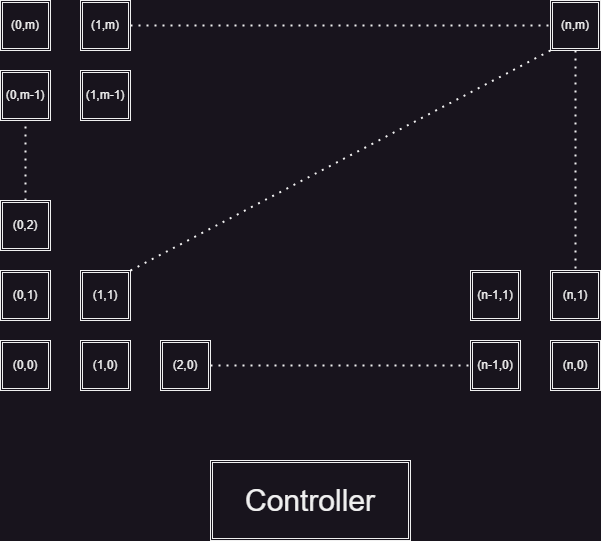
\includegraphics[width=11cm]{Images/CGoLDesign.png}
       \caption{Design of System for Conway's Game of Life}
           \label{fig:ProteusCGoLDesign}
\end{figure}

There will be two types of state machines: The cell, and the controller.
I will now describe the data associated with each state machine.

The cell has 5 local variables:
\begin{enumerate}[leftmargin=4\parindent]
    \item myName: the name of the cell as a string. (Final)
    \item Xcoord: the x coordinate as an integer. (Final)
    \item Ycoord: the y coordinate as an integer. (Final)
    \item currCellIsOn: holds the value of the current state of the cell (true == On).
    \item nextStateCurrCellIsOn: holds the value of the next state of the cell (true == On).
\end{enumerate}

Each cell also has 3 states: 
\begin{enumerate}[leftmargin=4\parindent]
    \item Display: broadcasts currState to whatever machine requested the current state of the cell.
    Is the initial state the cell is in.
    \item CalculateNext: Asks the neighbors in the 4 cardinal directions for their Display.
    Then determines based on the rules of CGoL what the next state of this cell should be.
    \item Update: updates currState to the value of nextStateCurrCellIsOn
\end{enumerate}

The controller is much simpler.
It has no local variables and only 2 states:

\begin{enumerate}[leftmargin=4\parindent]
    \item Setup: Determines cells to turn on/off when starting the program
    \item nextStep: broadcasts a message to all Cells to (1) calculate their next state and (2) update after finding their next state.
\end{enumerate}

\subsection{Implementation of Conway's Game of Life}

In total there are 4 events that will be used in the Proteus code:
\begin{enumerate}
    \item getDisplay(myName): the current cell requests another cell for their currState value.
    It passes the current cells name so that the receiver may transmit the data back to this cell.
    \item calculateNextState(): this event is sent from the controller to all cells.
    It instructs the cells to calculate their next state (true == On).
    \item updateAllCells(): this event is sent from the controller to all cells.
    It instructs the cells to update their currCellIsOn to the value of nextStateCurrCellIsOn.
    \item initializeCell(Value): this event is sent from the controller to all programmer-defined cells.
    It instructs the cell to update it's currCellIsOn to the given Value, with Value $\in$ \{true,false\}.
\end{enumerate}

The Proteus code for a given cell at coordinates (X,Y) are as follows:
(EN - if Proteus does not accept 'HSMName' to be defined dynamically, then instead add 4 vars to store the name of each of the neighbors statically. Another option would be to leave it outside of a variable and hardcode it)

\begin{verbatim}
actor cellXY{
    string myName = "cellXY";
    int Xcoord = [X];
    int Ycoord = [Y];
    bool currCellIsOn = false;
    bool nextStateCurrCellIsOn = false;
    statemachine {
        initial Display;
        state Display {
            on getDisplay {otherCellName} {otherCellName ! currCellIsOn}
            on calculateNextState {} {go calculateNext {}}
            on updateAllCells {} {go Update {}}
            on initializeCell {Value} {currCellIsOn = Value}
        }
        state calculateNext {
            int neighborTop = [Y]coord + 1;
            int neighborBot = [Y]coord - 1;
            int neighborLeft = [X]coord - 1;
            int neighborRight = [X]coord + 1;
            string neighborTopName = "cell" + Xcoord + neighborTop;
            string neighborBotName = "cell" + Xcoord + neighborBot;
            string neighborLeftName = "cell" + neighborLeft + Ycoord;
            string neighborRightName = "cell" + neighborRight + Ycoord;
            int count = 0;
            if (neighborTopName ! getDisplay {myName}) {
                count += 1;
            }
            if (neighborBotName ! getDisplay {myName}) {
                count += 1;
            }
            if (neighborLeftName ! getDisplay {myName}) {
                count += 1;
            }
            if (neighborRightName ! getDisplay {myName}) {
                count += 1;
            }
            if ((!(currCellIsOn)) && (count == 3)) {
                nextStateCurrCellIsOn = true;
            } else if ((currCellIsOn) && ((count == 2) || (count == 3))) {
                nextStateCurrCellIsOn = true;
            } else if ((currCellIsOn) && (count < 2)) {
                nextStateCurrCellIsOn = false;
            } else if ((currCellIsOn) && (count > 3)) {
                nextStateCurrCellIsOn = false;
            }
            go Display {}
        }
        state Update {
            currCellIsOn = nextStateCurrCellIsOn;
            go Display {}
        }
    }
}
\end{verbatim}

Assuming that there are a nonzero amount of cells that are to be initialized to a desired state, the Proteus code for the controller is as follows.
Let $cellXY, \dots, cellAB$ be the cells to be defined with initial states, and associated states $s0, \dots, sAB$.
In order to send an event to all the cells, I will write $cellSS, \dots, cellFF$ to represent the start and finishing cells in this list of possible cells.

\begin{verbatim}
actor controller{
    statemachine {
        initial Setup;
        state Setup {
            cellXY ! initializeCell { s0 };
            ...
            cellAB ! initializeCell { sAB };
            go nextStage {}
        }
        state nextStage {
            cellSS ! calculateNextState {};
            ...
            cellFF ! calculateNextState {};
            cellSS ! updateAllCells {};
            ...
            cellFF ! updateAllCells {};
        }
    }
}
\end{verbatim}

The only thing missing is to tell the controller how many times to repeat the next stage.
This is not a requirement for satisfying the capability of CGoL, but an extra nicety that would allow users to view the results at each stage.
As such, the above Proteus code demonstrates CGoL, and is verifiably TC as shown previously in section \ref{subsubsec:CGoL}.

\section{Creating Rule 110}\label{sec:ImplementRule110}

Another way to demonstrate that Proteus is TC is by implementing Rule 110.
I will similarly start by outlining the design of the program followed by the implementation in Proteus code.

\subsection{Design of the Program}

Recall Rule 110 in section \ref{subsubsec:Rule110}.
To represent the standard one-dimensional (1D) grid, I will use state machines for each cell.
To remain consistent, I will be simulating the 1D plane and assuming an arbitrary cell is the origin, 0.
This is to simplify referencing particular cells within the infinite 1D plane.

To begin, let there be a non-zero amount of cells that are to be initialized to some starting state.
I will define the bounds of the grid of initialized cells with $n \in \mathbb{N}$.
Each cell will be labeled with it's respective position according to the origin, 0.

Figure \ref{fig:ProteusRule110Design} illustrates the design of the line with each of the cells.
Note that I have only depicted the cells within the first n cells because these are the cells where the initialization process is described.

Similar to demonstarting CGoL seen in the previous section, there is also a 'Controller' which is not a part of this 1D plane but is capable of interacting with all cells in Figure \ref{fig:ProteusRule110Design}.
All the cells within the plane will be state machines, alongside this 'Controller'.

\begin{figure}[htb]
    \centering
    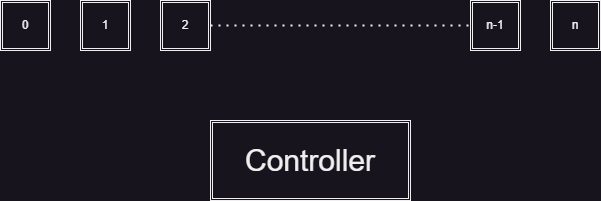
\includegraphics[width=11cm]{Images/Rule110Design.png}
       \caption{Design of System for Rule 110}
           \label{fig:ProteusRule110Design}
\end{figure}

There will be two types of state machines: The cell, and the controller.
I will now describe the data associated with each state machine.

The cell has 4 local variables:
\begin{enumerate}[leftmargin=4\parindent]
    \item myName: the name of the cell as a string. (Final)
    \item coord: the coordinate of the cell as an integer. (Final)
    \item currCellIsOn: holds the value of the current state of the cell (true == On).
    \item nextStateCurrCellIsOn: holds the value of the next state of the cell (true == On).
\end{enumerate}

Each cell also has 3 states: 
\begin{enumerate}[leftmargin=4\parindent]
    \item Display: broadcasts currState to whatever machine requested the current state of the cell.
    Is the initial state the cell is in.
    \item CalculateNext: Asks the adjacent neighbors for their Display.
    Then determines based on the rules of Rule 110 what the next state of this cell should be.
    \item Update: updates currState to the value of nextStateCurrCellIsOn
\end{enumerate}

The controller is simpler.
It has no local variables and only 2 states:

\begin{enumerate}[leftmargin=4\parindent]
    \item Setup: Determines cells to turn on/off when starting the program
    \item nextStep: broadcasts a message to all Cells to (1) calculate their next state and (2) update after finding their next state.
\end{enumerate}

\subsection{Implementation of the Rule 110}

In total there are 4 events that will be used in the Proteus code:
\begin{enumerate}
    \item getDisplay(myName): the current cell requests another cell for their currState value.
    It passes the current cells name so that the receiver may transmit the data back to this cell.
    \item calculateNextState(): this event is sent from the controller to all cells.
    It instructs the cells to calculate their next state (true == On).
    \item updateAllCells(): this event is sent from the controller to all cells.
    It instructs the cells to update their currCellIsOn to the value of nextStateCurrCellIsOn.
    \item initializeCell(Value): this event is sent from the controller to all programmer-defined cells.
    It instructs the cell to update it's currCellIsOn to the given Value, with Value $\in$ \{true,false\}.
\end{enumerate}

The Proteus code for a given cell at coordinate X are as follows:
(EN - if Proteus does not accept 'HSMName' to be defined dynamically, then instead add 2 vars to store the name of each of the neighbors statically. Another option would be to leave it outside of a variable and hardcode it)

\begin{verbatim}
actor cellXY{
    string myName = "cellX";
    int coord = [X];
    bool currCellIsOn = false;
    bool nextStateCurrCellIsOn = false;
    statemachine {
        initial Display;
        state Display {
            on getDisplay {otherCellName} {otherCellName ! currCellIsOn}
            on calculateNextState {} {go calculateNext {}}
            on updateAllCells {} {go Update {}}
            on initializeCell {Value} {currCellIsOn = Value}
        }
        state calculateNext {
            int neighborLeft = coord - 1;
            int neighborRight = coord + 1;
            string neighborLeftName = "cell" + neighborLeft;
            string neighborRightName = "cell" + neighborRight;
            bool valNeighborLeft = neighborLeftName ! getDisplay {myName};
            bool valNeighborRight = neighborRightName ! getDisplay {myName};
            if ((valNeighborLeft) && (currCellIsOn) 
                    && (valNeighborRight)) {
                nextStateCurrCellIsOn = false;
            } else if ((valNeighborLeft) && (currCellIsOn) 
                    && (!(valNeighborRight))) {
                nextStateCurrCellIsOn = true;
            } else if ((valNeighborLeft) && (!(currCellIsOn)) 
                    && (valNeighborRight)) {
                nextStateCurrCellIsOn = true;
            } else if ((valNeighborLeft) && (!(currCellIsOn)) 
                    && (!(valNeighborRight))) {
                nextStateCurrCellIsOn = false;
            } else if ((!(valNeighborLeft)) && (currCellIsOn) 
                    && (valNeighborRight)) {
                nextStateCurrCellIsOn = true;
            } else if ((!(valNeighborLeft)) && (currCellIsOn) 
                    && (!(valNeighborRight))) {
                nextStateCurrCellIsOn = true;
            } else if ((!(valNeighborLeft)) && (!(currCellIsOn)) 
                    && (valNeighborRight)) {
                nextStateCurrCellIsOn = true;
            } else {
                nextStateCurrCellIsOn = false;
            }
            go Display {}
        }
        state Update {
            currCellIsOn = nextStateCurrCellIsOn;
            go Display {}
        }
    }
}
\end{verbatim}

Assuming that there are a nonzero amount of cells that are to be initialized to a desired state, the Proteus code for the controller is as follows.
Let $cellX, \dots, cellY$ be the cells to be defined with initial states, and associated states $s1, \dots, sN$.
In order to send an event to all the cells, I will write $cellS, \dots, cellF$ to represent the start and finishing cells in this list of possible cells.

\begin{verbatim}
actor controller{
    statemachine {
        initial Setup;
        state Setup {
            cellX ! initializeCell { s1 };
            ...
            cellY ! initializeCell { sN };
            go nextStage {}
        }
        state nextStage {
            cellS ! calculateNextState {};
            ...
            cellF ! calculateNextState {};
            cellS ! updateAllCells {};
            ...
            cellF ! updateAllCells {};
        }
    }
}
\end{verbatim}

The only thing missing is to tell the controller how many times to repeat the next stage.
This is not a requirement for satisfying the capability of Rule 110, but an extra nicety that would allow users to view the results at each stage.
As such, the above Proteus code demonstrates Rule 110, and is verifiably TC as shown previously in section \ref{subsubsec:Rule110}.

With this, I have concluded showing that Proteus is TC with 3 verified methods:
\begin{enumerate}
    \item Constructing a TM with an undecidable input
    \item Implementing Conway's Game of Life in a Proteus program
    \item Implementing Rule 110 in a Proteus program
\end{enumerate}